\documentclass[status=normal,cover=tesi,language=en]{gmeepd}

\ShowDraft 

% --- definizione copertina ---------------------------------------------------------------
%% definizione elementi che compongono la copertina
%\renewcommand{\CoverType}{elaborato} % default elaborato, altri possibili: tesina, tesi, dispensa, libro, mycover (vedere istruzioni più avanti)
%\renewcommand{\CoverType}{elaborato}
% default elaborato, altri possibili: tesina, tesi, tesiphd, dispensa, libro

\Author{Marco Martini}
\Title{Managing Security of Computer Network Applications using Encryption Techniques}
%\Subtitle{tesi}
\Advisor{ Professor Dr. Ing. Nicola Laurenti}
\CoAdvisor{Professor Dr. Ing. Alexandru Soceanu}
\Course{corso di laurea in Ingegneria Informatica}
\Date{\today}   % default=\today

% -------------------------------------------------------------------------------------------

\makeindex % chiede a LaTeX di creare l'indice analitico, la stampa (opzionale) avviene in fondo

\usepackage{glossaries}
\usepackage[skip=1ex]{caption}
\usepackage{listings}
\lstset{basicstyle=\ttfamily,
  showstringspaces=false,
  commentstyle=\color{red},
  keywordstyle=\color{blue}
}


\makeglossaries % Glossario per latex

\begin{document}

\Cover    % copertina

\tableofcontents

\printglossaries


\chapter{Abstract}
\section{English}

This paper covers the usage of SSL and TLS encryption techniques to improve the security of the Computer Network applications including their weaknesses. In order to do that an HTTPS web server will be implemented and will be accessed through a virtual network.
The virtual network will be protected through a proprietary Next Generation Firewall (NGFW) from Palo Alto Networks, the paper will explore its Malware Detection and SSL Decryption capabilities showing their advantages and/or weaknesses.
In order to verify the Firewall's effectiveness a Man In The Middle (MITM) attack will be deployed inside the virtual network.
This paper will end by stating the results obtained by analyzing the NGFW tools and their behaviour against the network attacks.

\section{Italian}

Questo documento copre l'utilizzo di tecniche di cifratura SSL e TLS per aumentare la sicurezza di applicazioni di rete rimediando alle loro vulnerabilit\`a.
Per farlo verr\`a creata una rete virtuale che acceder\`a ad un server web HTTPS.
La rete virtuale sar\`a protetta dal Firewall di nuova generazione (NGFW) proprietario di Palo Alto Networks, esplorando le funzionalit\`a di Malware Detection e SSL Decryption, elencandone i vantaggi e/o svantaggi.
Per dimostrare l'efficacia del Firewall verr\`a creato un attacco Man In The Middle (MITM).
Si dimostrano infine i risultati dell'esperimento dati dall'analisi del comportamento degli strumenti del Firewall contro gli attacchi di rete.


\chapter{Introduction}
\section{Motivation for the Work}

During the past 30 years the way we use computers has fundamentally changed, we now have devices capable of connecting to the Internet in our pockets, and that has lead to an ever increasing interest for companies to focus on the Web.

Nowadays the 55.9\% of Alexa's list of most popular sites in the world provide a Secure SSL/TLS implementation\cite{ssl-pulse}.

While Encryption provides Confidentiality and Integrity\cite{ibm-ssl} for the end user, it also provide attackers and malware software a way to inject their payload to vulnerable clients without being able to be detected.

This paper will be focused on the Malware protection capabilities that NGFW provide, even in encrypted connections. It's capable of that through an SSL Forward Proxy.

Despite the added security achieved by having a mediator between the untrusted zone (Internet) and the client, a Man In The Middle (MITM) attack could be used to compromise the network if forged well enough, this work will prove whether or not NGFW are effective against this type of attacks.


\section{Objective of the Work}

The Objective of this work will be showing how to implement a Decryption tunnel and Malware Detection in Palo Alto FW and demonstrating it's effectiveness when the network has been compromised through a MITM attack.

%It will also report how to mitigate the attack.

\section{Summary of the Work}

The Work will be as following:

\begin{itemize}
    \item Setting up the Virtual Network
    \item Setting up Palo Alto Firewall
    \item Setting up Malware Detection
    \item Creating the SSL/TLS Certificates
    \item Setting up Decryption
    \item Testing Malware Detection
    \item Setting up the MITM attack
    \item Testing Malware Detection again
    \item Setup a way to block the attack
\end{itemize}

\chapter{Description of the Components}

The following sections will briefly describe the components used in this experiment.

\section{Next Generation Firewalls and Palo Alto}

\subsection{Next Generation Firewalls}

Next Generation Firewalls are the evolution of traditional firewalls and are bound to replace them entirely in the corporate space.

Traditional Firewalls can only filter traffic based on state (flow of data instead of single network packets), port, protocol or through hand crafted filters.

Even if a Traditional Firewall is aware of the state of the connection, the data it can extrapolate is very low, for example it knows:

\begin{itemize}
 \item When was the flow started
 \item When the flow is being used
 \item When the flow is being closed
\end{itemize}

\pagebreak

A Next Generation Firewall does everything a Traditional Firewall can and more by using AI enhanced algorithms  and by using the Cloud as to always be up to date with new threats and malware.

In order for a Firewall to be classified as ``New Generation'' it must provide(source: ``https://www.cisco.com/c/en/us/products/security/firewalls/what-is-a-next-generation-firewall.html\#~choose-an-ngfw-firewall''):

\begin{itemize}
 \item Standard firewall capabilities like stateful inspection
 \item Integrated intrusion prevention
 \item Application awareness and control to see and block risky apps
 \item Threat intelligence sources
 \item Upgrade paths to include future information feeds
 \item Techniques to address evolving security threats
\end{itemize}

\pagebreak

\subsection{Palo Alto Firewalls}

Palo Alto Networks is an American multinational cybersecurity company based in Santa Clara, California.

Other than the mandatory NGFW features, Palo Alto's Firewall solutions provide many more tools, some of which are\cite{panos-features}:

\begin{itemize}
    \item Application-based policy enforcement (App-ID?)
    \item User identification (User-ID?).
    \item Threat prevention.
    \item URL filtering.
    \item Traffic visibility.
    \item Networking versatility and speed.
    \item GlobalProtect.
    \item Fail-safe operation.
    \item Malware analysis and reporting.
    \item VM-Series firewall.
    \item Management and Panorama.
\end{itemize}

This paper will cover the Threat analysis feature of this platform enhanced by the decryption of SSL/TLS packets.

\pagebreak

\section{SSL/TLS Decryption}

SSL and TLS protocols are the most used protocols to provide secure communication over the internet.

They are present between the Application Layer and the Transport Layer in the TCP/IP stack and enable to identify and authenticate two parties by keeping confidentiality and data integrity.

\begin{figure}[!hb]
    \centering
    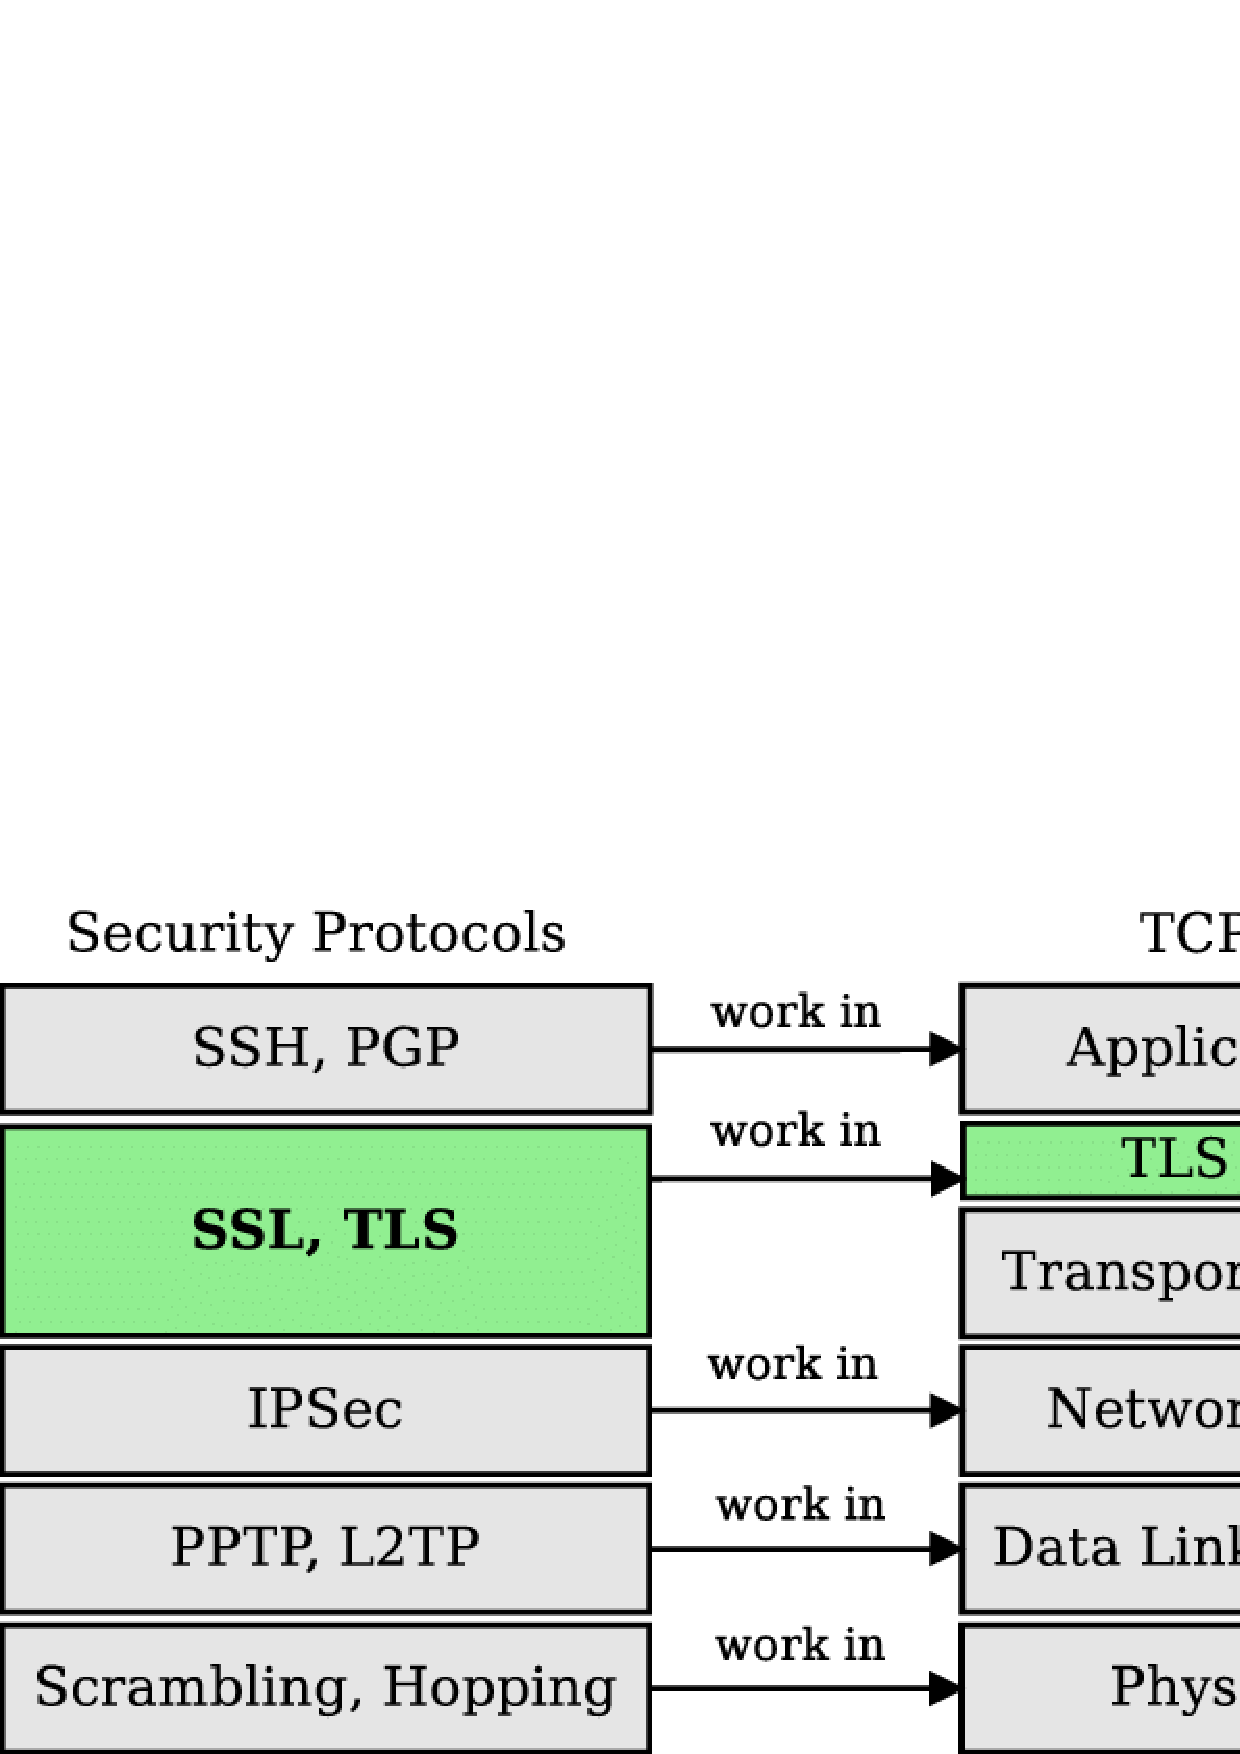
\includegraphics[width=13cm]{img/ssl-stack.png}
    \caption{The SSL Layer in the TCP/IP Stack}
    \label{SSL Layer}
\end{figure}


\pagebreak

In order for the two parties to communicate, an SSL/TLS Handshake must be performed first.


\begin{figure}[!hb]
 \centering
 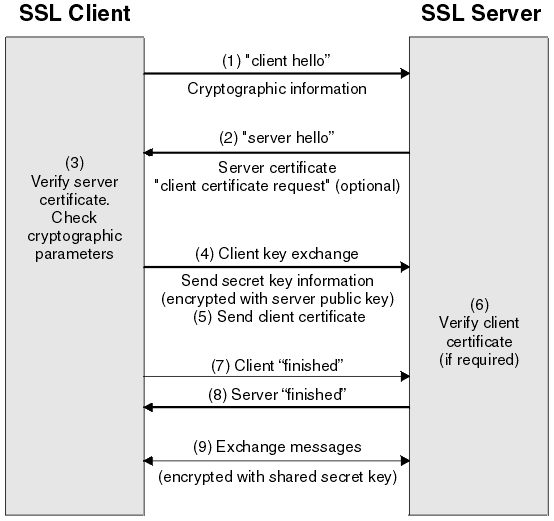
\includegraphics[width=13cm]{img/ssl_handshake.png}
 \caption{Overview of the SSL or TLS handshake}
 \caption*{Source: https://www.ibm.com/docs/en/ibm-mq/7.5?topic=ssl-overview-tls-handshake}
 \label{SSL handshake}
\end{figure}

In short the first two packets are needed to establish the role of client/server between the two parties and establish a supported Cipher and Compression method along with the server sending the digital certificate.

After that the client verifies the server's certificate, sends a secret key used to encrypt the following data which is encrypted itself with the server's public key and optionally sends its own certificate in case of a symmetrical encryption method.

Finally both the client and server send a ``finished'' message encrypted with the secret key indicating that the handshake is complete.

The SSL Decryption covered in this paper refers as a technique where instead of having  2 parties, we have 3:

The server establishes a handshake with the firewall acting as a client and the firewall at the same time establishes an handshake to the real client by acting as the server.

\begin{figure}[!hb]
 \centering
 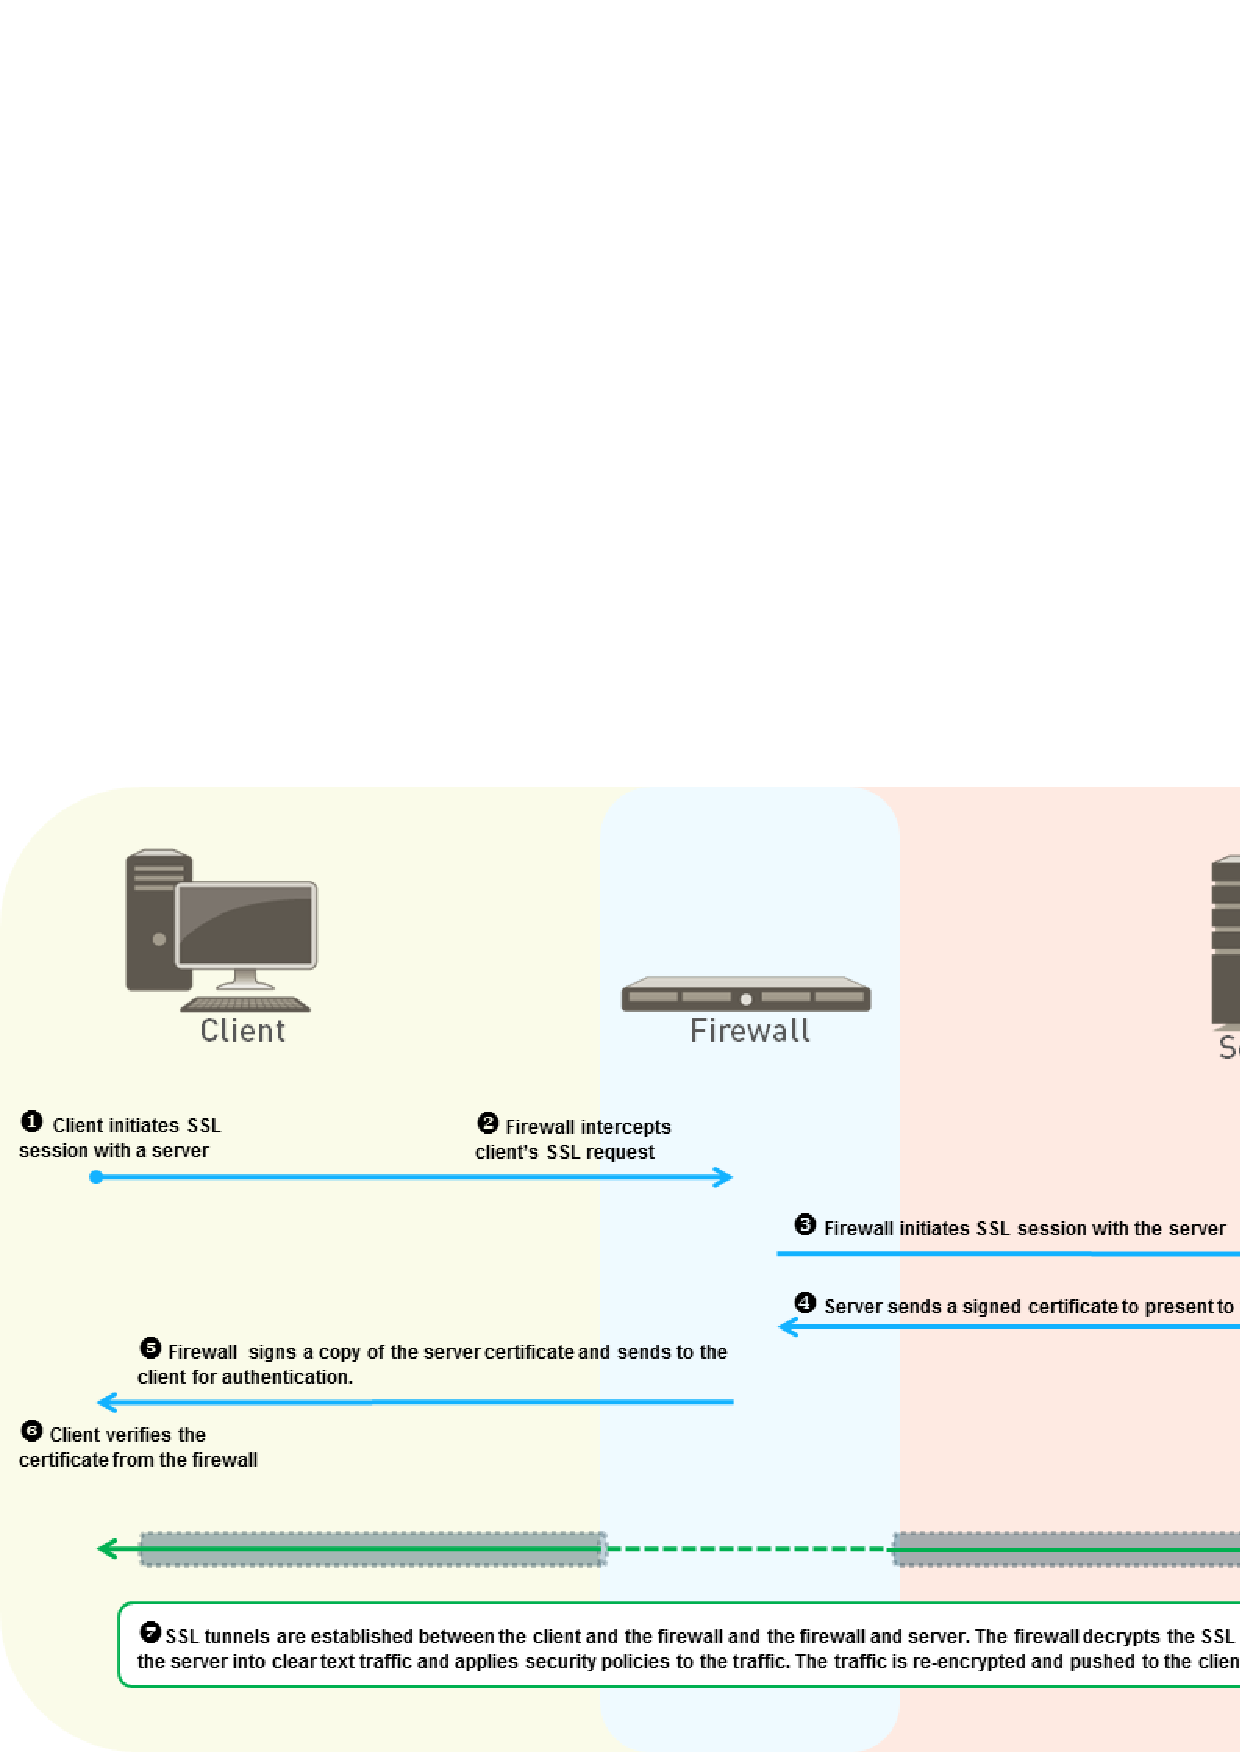
\includegraphics[width=13cm]{img/ssl_decryption_diagram.png}
 \caption{SSL Forward Proxy Diagram}
 \caption*{Source: https://www.ibm.com/docs/en/ibm-mq/7.5?topic=ssl-overview-tls-handshake}
 \label{SSL Forward Diagram}
\end{figure}

\pagebreak

\section{Malware Detection in Firewalls}

The first line of protection in an organization against malicious attackers is in most cases the Firewall.

Since a Firewall provides a gateway to the outside world it makes sense that a malware protection strategy will also be installed there.

Traditional Firewalls used to only be able to inspect a flow of non-encrypted data, as such, the only way to detect malware was to compare the hash of the downloaded data from the client to a local database which is highly exploitable (by for example changing a few bytes in the payload).

Through NGFWs Malware signatures can be constantly updated through the Cloud and instead of comparing hashes, the threat prevention in this new technology can analyse the payload itself, even if compressed or comes from an encrypted source such as HTTPS.

\section{HTTPS Server with Let's Encrypt}

The HTTPS protocol is a secure version of the HTTP, to make it secure, SSL/TLS certificates must be installed into the server that deploys it.

Let's Encrypt is a non-profit Certification Authority that provides TLS certificates for free, although valid for only 90 days.

The official implementation is `certbot`, a tool that automates the generation and renewal of the certificates.

It also provide an automatic certificate installation for `nginx` and `Apache`, the most popular and Open Source web server software.

\section{The Network Attack}

Since SSL Decryption is just a Man in The Middle implementation, the web client must trust the firewall before the website, so if not careful an user can be a victim of another MITM implementation.

\pagebreak

\subsection{ARP Spoofing}

In order to deploy a successful MITM attack the user must connect to the Attacker machine first.

ARP Spoofing, or ARP poison, consists in a technique where the attacker sends multiple spoofed ARP messages.

Since ARP, Address Resolution Protocol, is used to associate a network device MAC address with its IP-address, spoofing an ARP message means that the attacker will forcefully associate the MAC address of the LAN Gateway to the machine of the attacker himself.

\begin{figure}[h!]
 \centering
 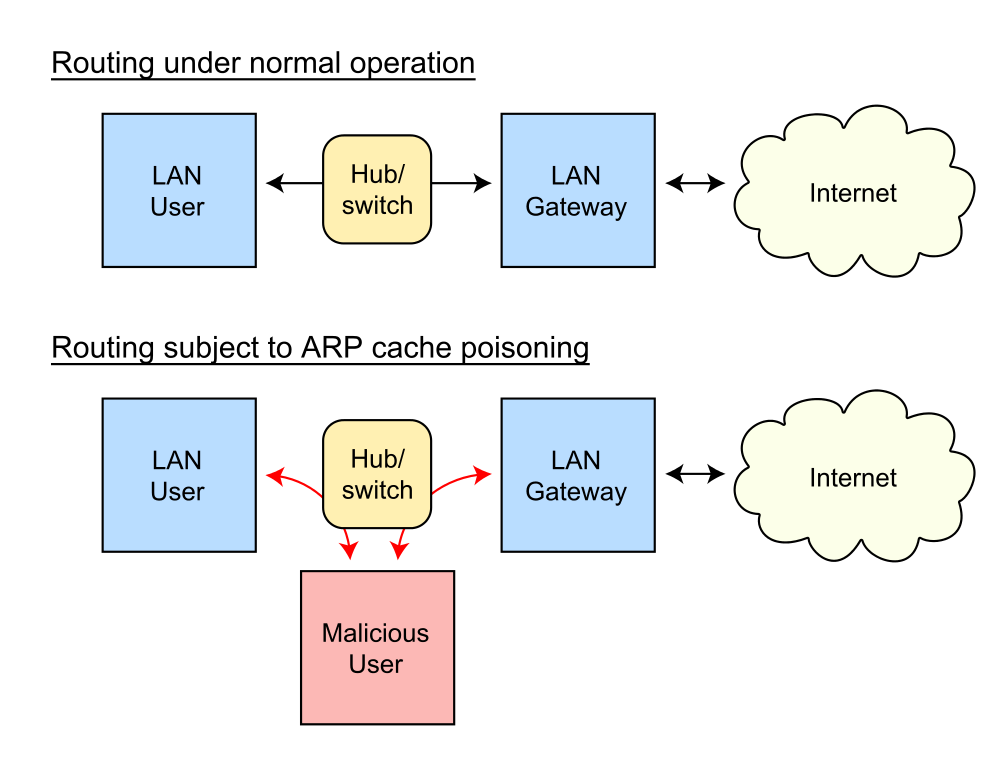
\includegraphics[width=13cm]{img/ARP_Spoofing.png}
 % ARP_Spoofing.png: 1005x768 px, 72dpi, 35.45x27.09 cm, bb=
 \caption{A successful ARP spoofing (poisoning) attack allows an attacker to alter routing on a network, effectively allowing for a man-in-the-middle attack}
 \caption*{Source: https://en.wikipedia.org/wiki/ARP\_spoofing}
 \label{fig: ARP Spoofing}
\end{figure}

\pagebreak

\subsection{HTTPS Proxy}

An HTTPS proxy is a server application that acts as an intermediary between a client and a SSL encrypted website.

If used together with a spoofer, in our case an ARP Spoofer, every HTTPS traffic in the network will be redirected to the attacker allowing them to modify the resource at will.

It works exactly like an HTTPS server so it also needs its own SSL/TLS certificates, when used in a Network Attack they're usually forged to seem legitimate.

\begin{figure}[h!]
 \centering
 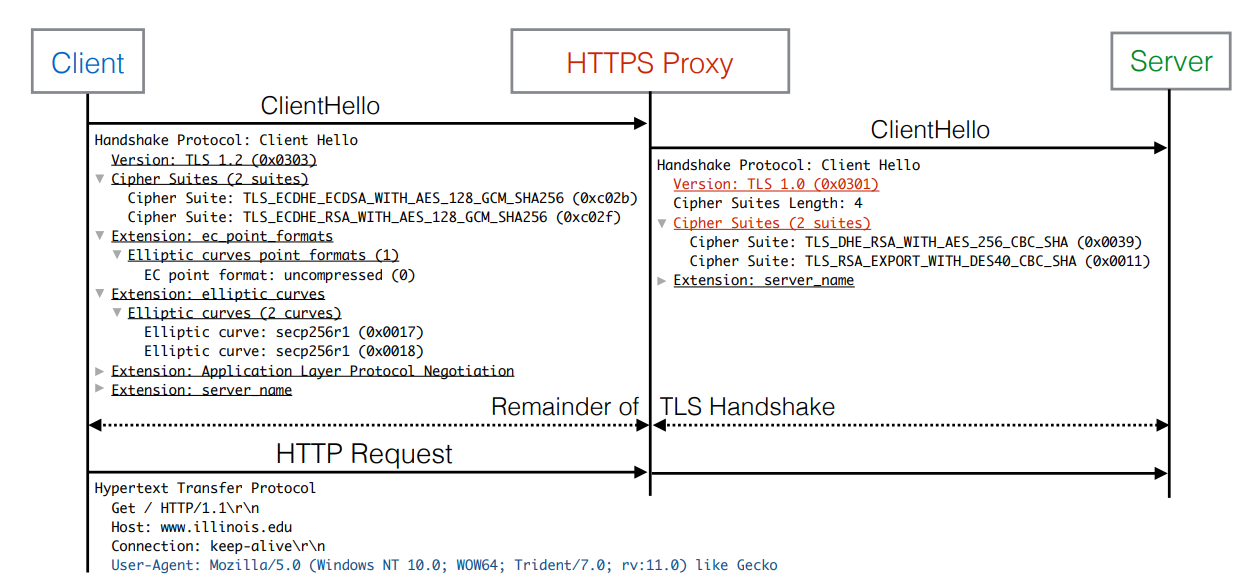
\includegraphics[width=13cm]{img/https_proxy_interception.png}
 % https_proxy_interception.png: 1255x583 px, 96dpi, 33.20x15.42 cm, bb=
 \caption{HTTPS Proxy Interception\protect\cite{https-interception}}
 \label{fig: HTTPS Proxy Interception}
\end{figure}


\chapter{The Experiment}
\section{Methodology}

In order to verify the firewall effectiveness a virtual laboratory will be setup.

The virtual laboratory is deployed through Virtual Machines, since the Palo Alto Firewall is very resource intensive the hypervisor of choice has been KVM(source), with libvirt/qemu as the userspace component.

Instead of direct access to the Internet the VM clients will connect to the host machine, the host will run NGINX(source) configured with Let's Encrypt(source) certificates as the HTTPS server, it will host a simple web page with a link that points to malware.

\begin{figure}[h!]
 \centering
 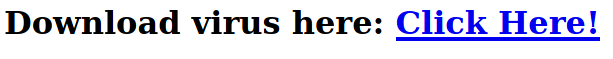
\includegraphics[width=13cm]{img/webpage.png}
 % webpage.png: 613x59 px, 96dpi, 16.22x1.56 cm, bb=
 \caption{The web page the client will connect to}
 \label{fig: webpage}
\end{figure}

\begin{verbatim}
 <html>
    <body>
        <h1>Download virus here:
            <a href="./eicar.com">
                Click Here!
            </a>
        </h1>
    </body>
</html>
\end{verbatim}

\begin{center}
The Source Code of the web page
\end{center}


The Malware in question is a test file created by ``eicar.org'', the European Institute for Computer Antivirus Research, which is purposely made to test the response of antivirus programs\cite{eicar}, in this case Palo Alto's Firewall.

The 2 Firewall clients on the other hand will be running  Kali Linux, an operating system designed for penetration testing, since it comes preinstalled with many tools.

The 2 clients have different purposes, one will be used as a standard client and the other as a malicious intruder which will deploy the network attack.

\begin{figure}[h!]
 \centering
 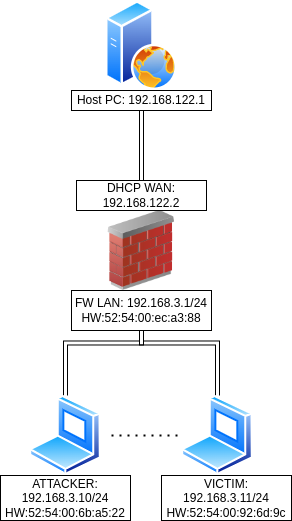
\includegraphics[height=13cm]{img/Network_Plan.png}
 % Network_Plan.png: 292x521 px, 72dpi, 10.30x18.38 cm, bb=
 \caption{The Network Plan}
 \label{fig: network-plan}
\end{figure}



\pagebreak

\section{Setting up the Firewall}

The first thing to do would be setting up the Firewall.

Since it's a simple network the firewall was setup with only 2 network interfaces, a WAN connected interface (in this case the host) and a LAN connected interface, where the clients are connected.

\begin{figure}[!hb]
 \centering
 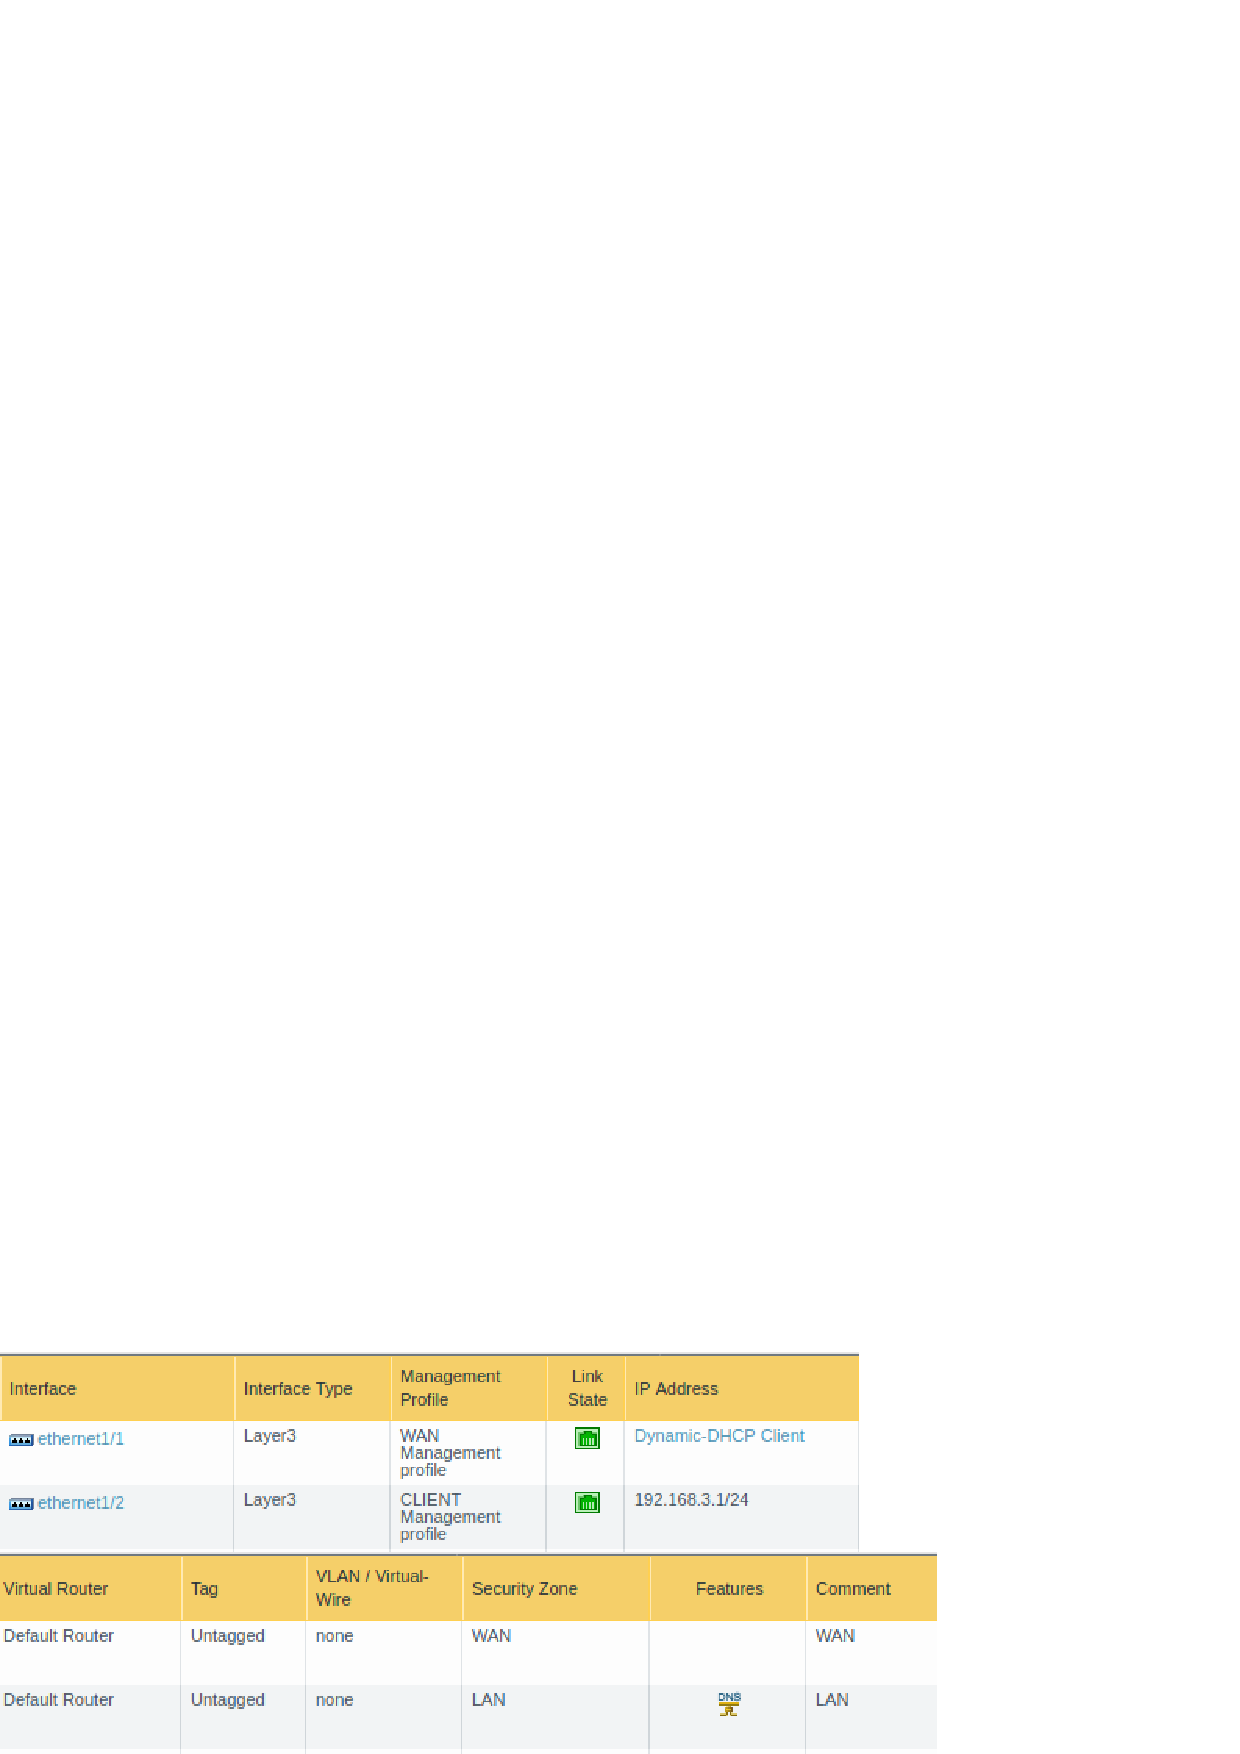
\includegraphics[width=13cm]{img/network_config.png}
 % network_config.png.eps: 874x111 px, 72dpi, 30.83x3.92 cm, bb=0 0 874 111
 \caption{The Network Interfaces' Configuration in Palo Alto FW}
 \label{Network Interfaces Configuration}
\end{figure}


The two interfaces must be configured to be part of a Virtual Router, so that the packets can be forwarded to each other.

\begin{figure}[!hb]
 \centering
 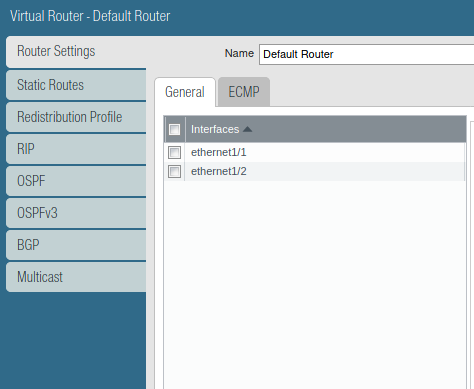
\includegraphics[width=13cm]{img/virtual_router.png}
 % virtual_router.png.eps: 600x373 px, 72dpi, 21.17x13.16 cm, bb=0 0 600 373
 \caption{The Virtual Router Configuration in Palo Alto FW}
 \label{Virtual Router Configuration}
\end{figure}


We need to create some policies in order for the inside network to reach the WAN area.

\begin{figure}[!hb]
 \centering
 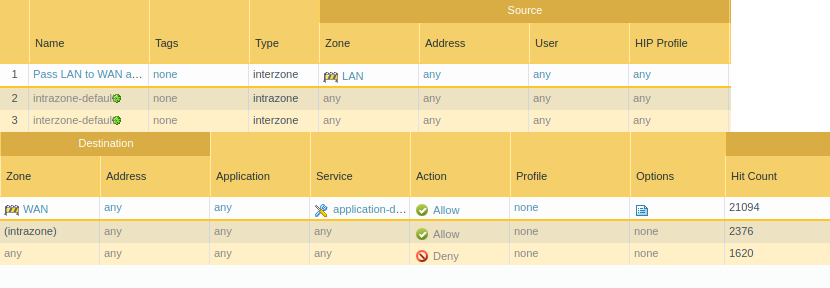
\includegraphics[width=13cm]{img/Firewall_Policy.png}
 % Firewall_Policy.png.eps: 622x216 px, 72dpi, 21.94x7.62 cm, bb=
 \caption{The Firewall Policies in Palo Alto FW}
 \label{Firewall Policies}
\end{figure}


Since the hosts outside of the internal network have no way to know where the source address is coming from, the next step is configuring NAT Masquerading, It's a technique in which IP addressed are mapped from one realm to another, in this case from the internal network to the external one and vice-versa(source:``https://www.rfc-editor.org/rfc/rfc2663.txt'').

\begin{figure}[!hb]
 \centering
 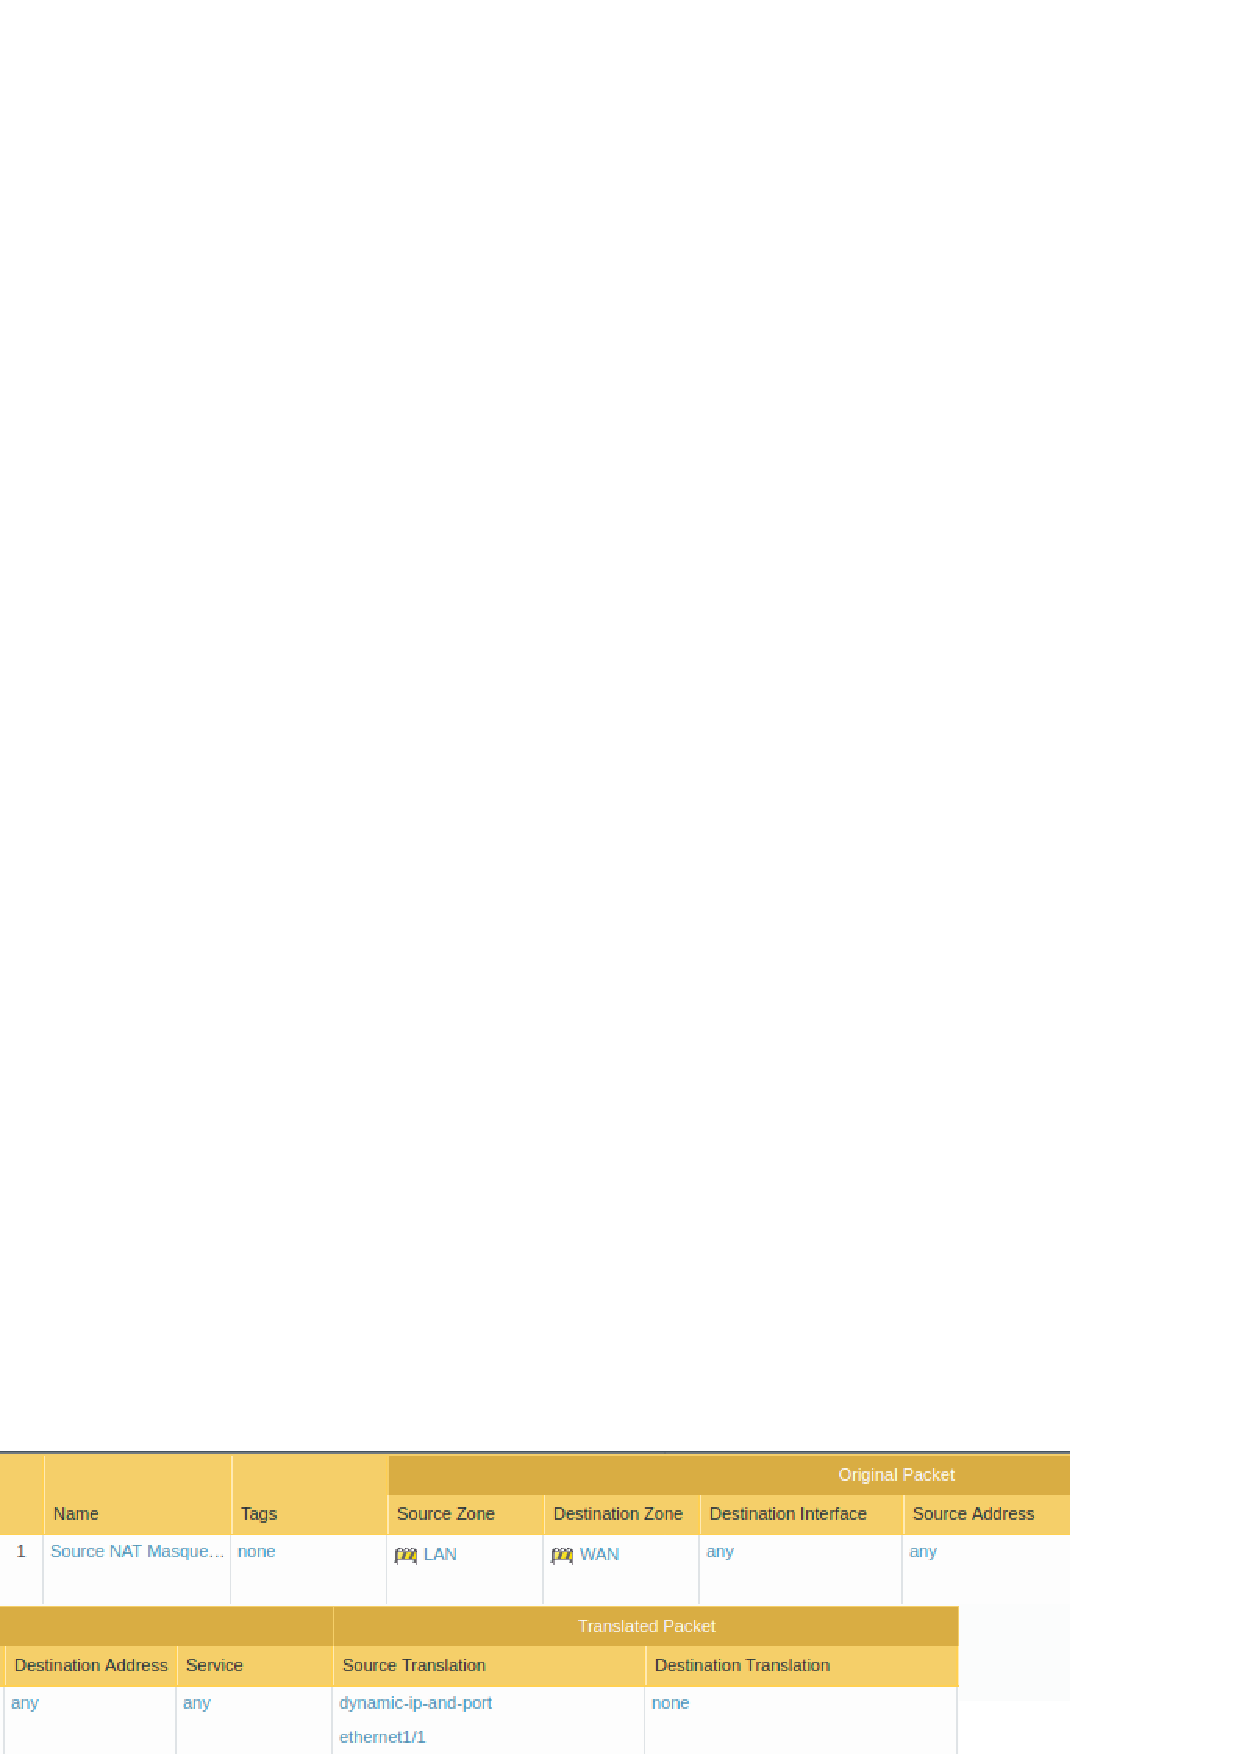
\includegraphics[width=13cm]{img/NAT_Masquerade.png}
 % NAT_Masquerade.png.eps: 514x145 px, 72dpi, 18.13x5.12 cm, bb=
 \caption{NAT Masquerading in Palo Alto FW}
 \label{NAT Masquerade}
\end{figure}


\pagebreak

\section{Setting up Decryption}

After the firewall has been configured, much like NAT works, the firewall stands in the middle between outbound and inbound connections.

The firewall connects to the server as the client would, representing it, and uses its own certificates to encrypt the connection between itself and the client making it so that the client believes to communicate directly with the server in a transparent way.

In order to do that we must generate our self signed certificate, and enable the option to Forward Trusted and/or Untrusted Certificates.

\begin{figure}[!hb]
\centering
 \subfloat[The Certificate Generation Menu in Palo Alto FW\label{Certificate Generation}]{
 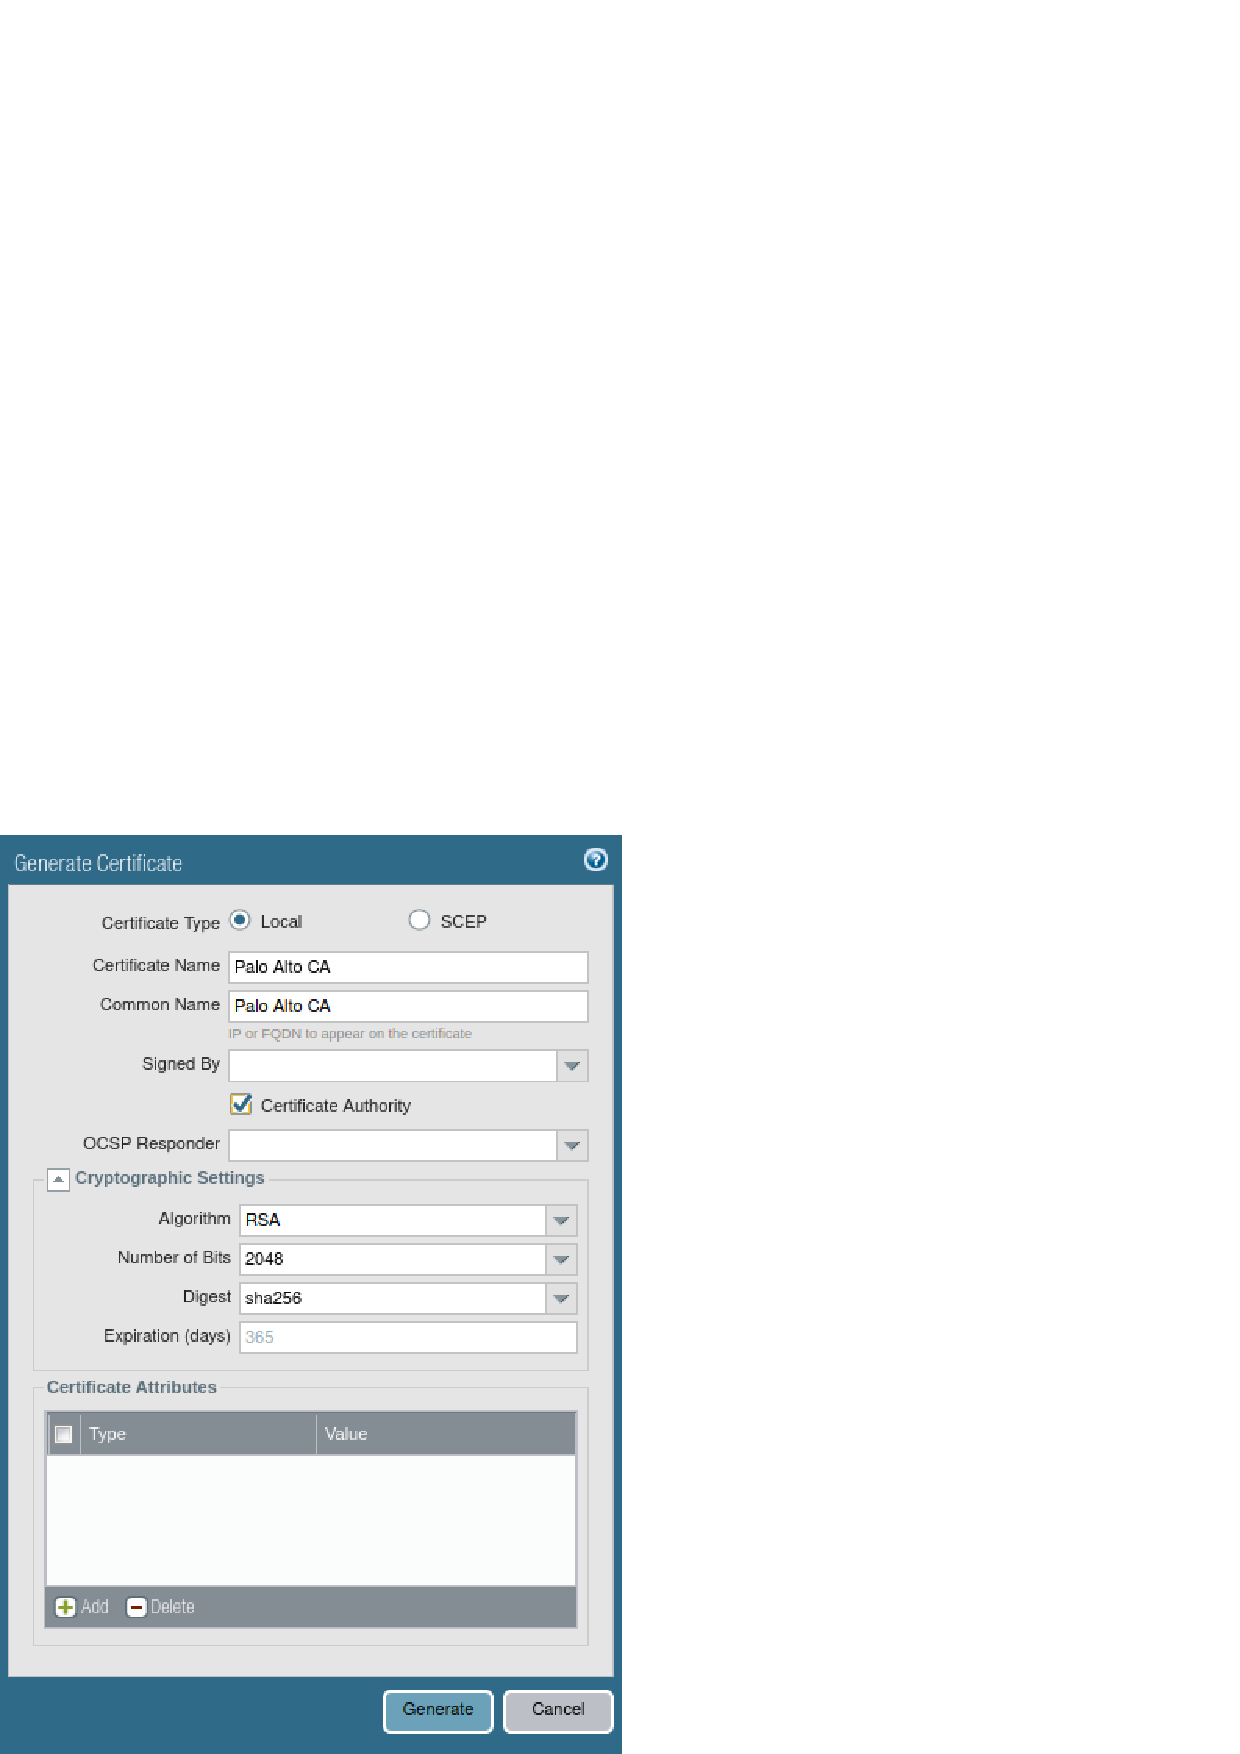
\includegraphics[width=6cm]{img/Certificate_generation.png}}
 \hspace{0.5cm}
 \subfloat[The Certificate Settings Menu in Palo Alto FW\label{Certificate Settings}]{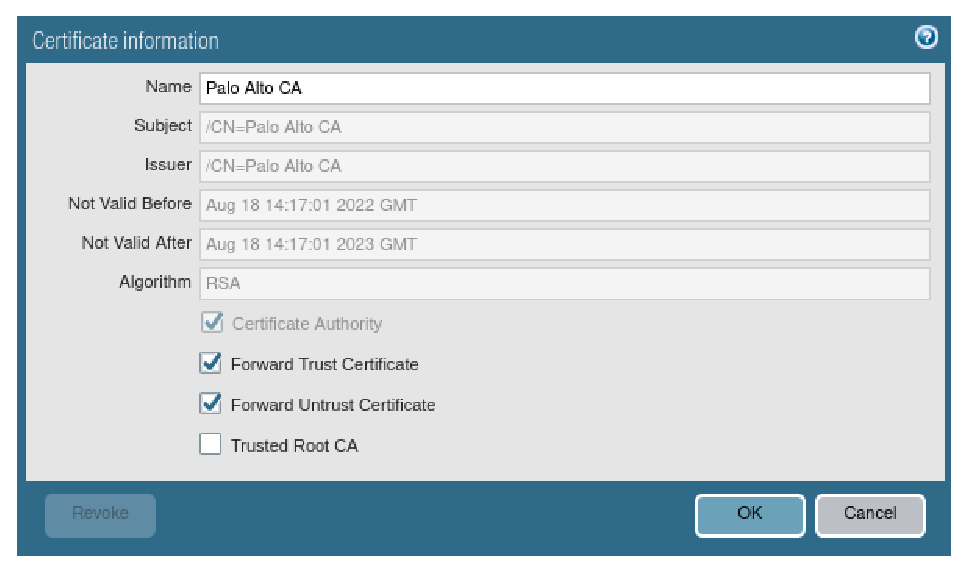
\includegraphics[width=6cm]{img/Certificate_settings.png.eps}}
 \caption{SSL/TLS Certificates configuration in PanOS}\label{Certificates}
\end{figure}

\pagebreak

After the Certificate Generation we need to have a working Decryption Profile, Palo Alto Firewall provides by default a working one but one could create a customised one if needed.

\begin{figure}[!hb]
    \centering
     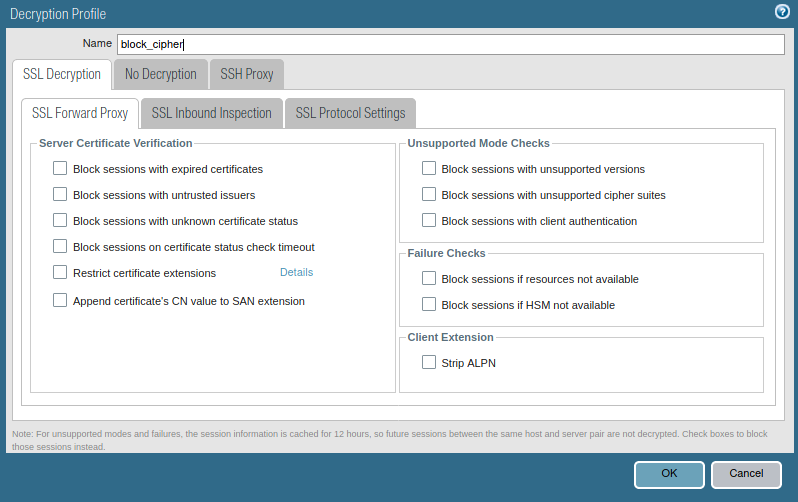
\includegraphics[width=13cm]{img/decryption_options.png}
    	\caption{A few of the many options configurable for Decryption}\label{Decryption Options}
\end{figure}

\pagebreak

Finally we can create a Decryption Policy, as with every other Firewall Policy, the source and Destination traffic must be selected, in this case any type of traffic, and then the decryption policy option, there are 3 types of Decryption available in Palo Alto FW: \verb|SSL Forward Proxy|, \verb|SSL Inbound Inspection|, \verb|SSH Proxy|

In this case an SSL Forward Proxy will be used as it's a general approach which works for every SSL/TLS based server without any need to import the private key from external servers.

\begin{figure}[!hb]
\centering
 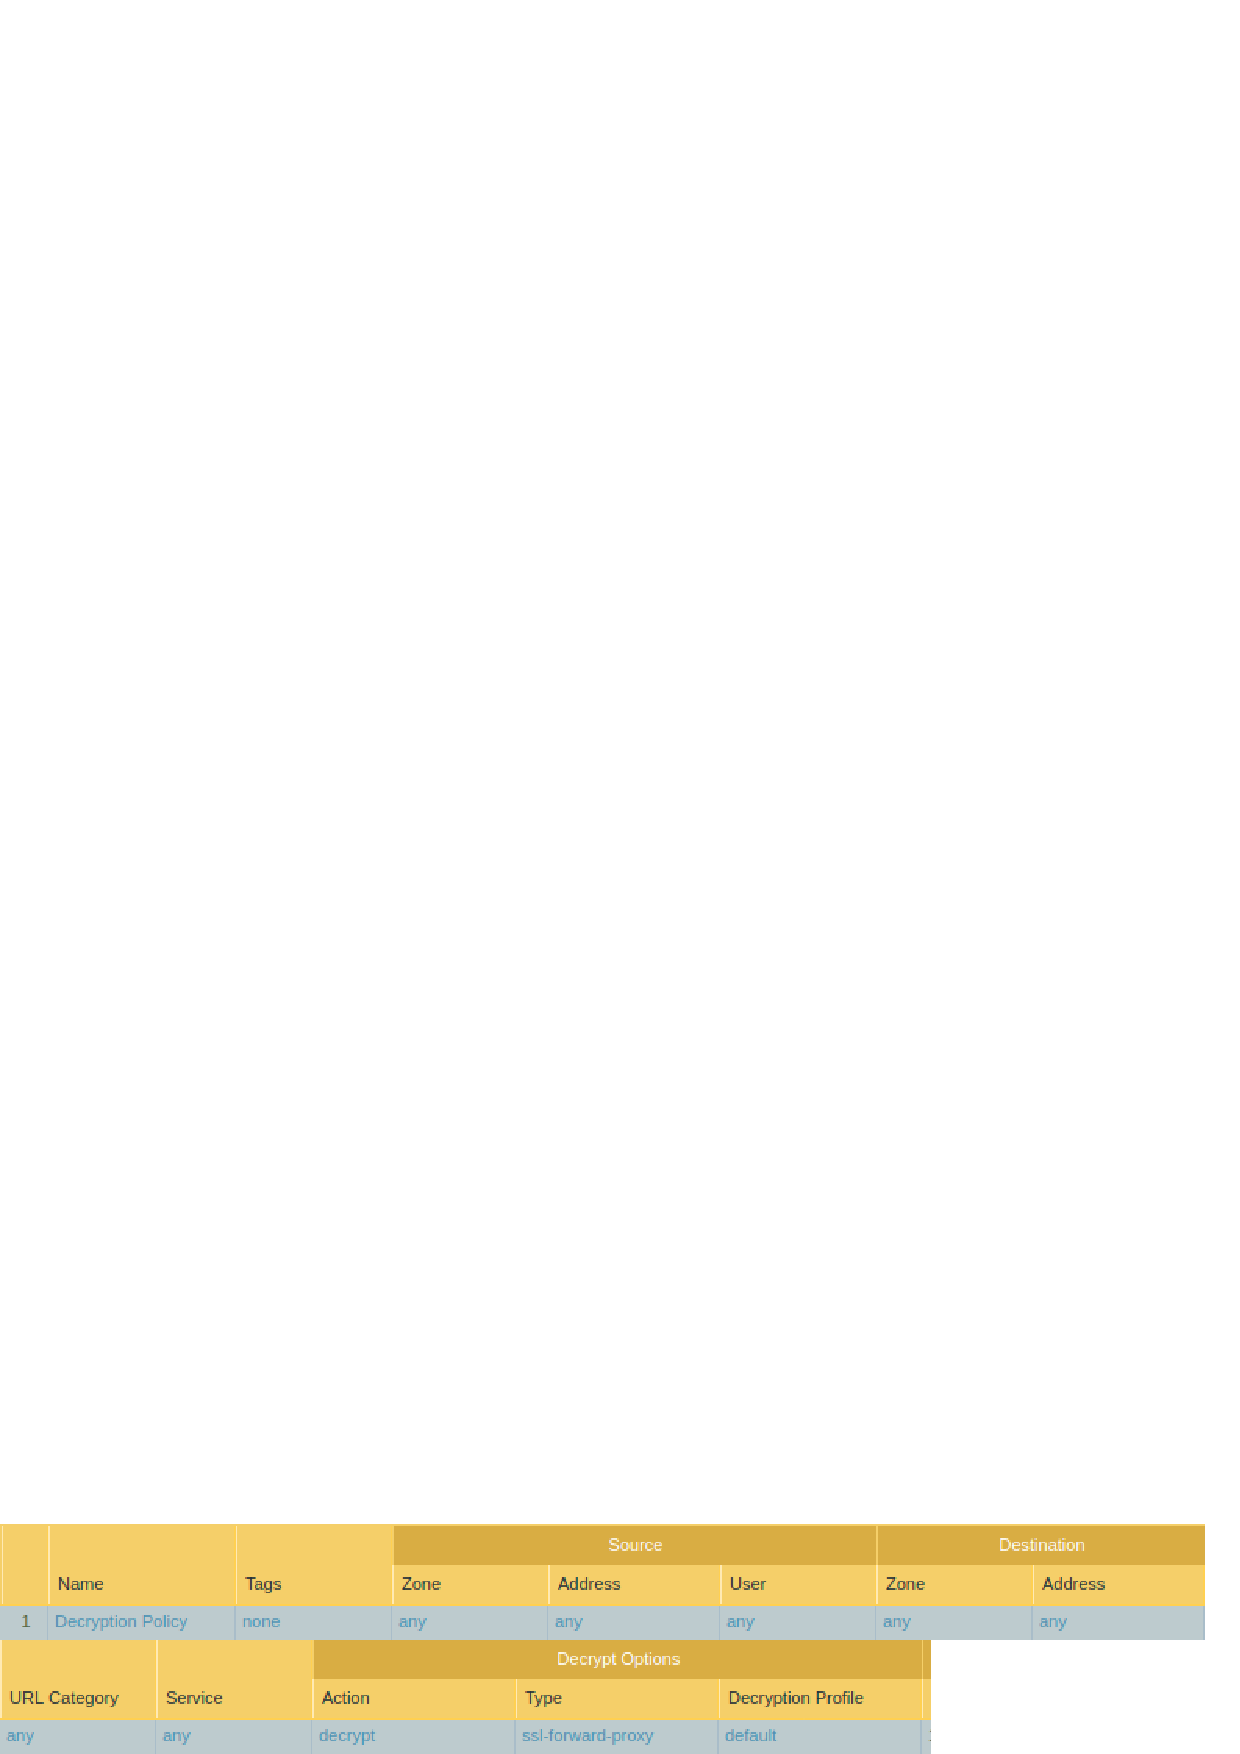
\includegraphics[width=13cm]{img/decryption_policy.png}
	\caption{Brief overview of the Decryption Policy used}\label{Decryption Policy}
\end{figure}

It's also possible to define some exceptions where the website included in it won't ever be decrypted, in case of trusted websites or when the website policy doesn't allow this form of redirection, for example when HSTS (HTTP Strict Transport Security) is enabled.

\begin{figure}[!h]
\centering
 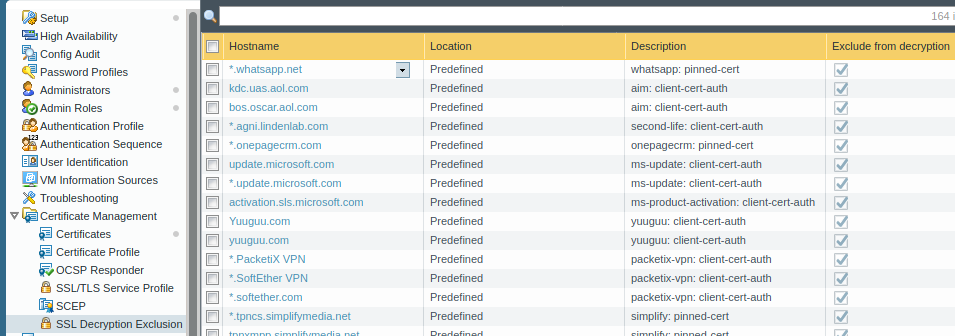
\includegraphics[width=12cm]{img/decryption_exceptions.png}
	\caption{A list of Decryption Exceptions}\label{Decryption Exceptions}
\end{figure}

\pagebreak

To verify if SSL Decryption is working correctly, after connecting to an HTTPS enabled website, this Captive Portal web page should show up before being able to connect.

\begin{figure}[!h]
\centering
 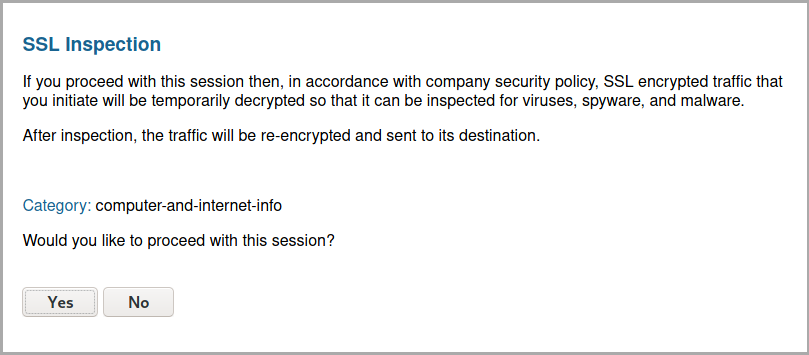
\includegraphics[width=13cm]{img/ssl_inspection_result.png}
	\caption{The SSL Inspection Captive portal }\label{SSL Inspection Page}
\end{figure}

It is also possible to look at the certificate used to decrypt the web page and verify that its Certificate Authority is the same as the one that was generated through the Firewall

\begin{figure}[h!]
 \centering
 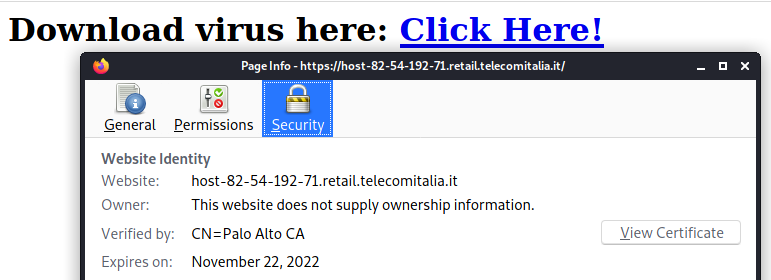
\includegraphics[width=13cm]{img/pa_certificate.png}
 % pa_certificate.png: 771x280 px, 96dpi, 20.40x7.41 cm, bb=
 \caption{The Palo Alto Generated Certificate on a foreign web page}
 \label{fig: PaloAlto certificate}
\end{figure}


\pagebreak

\section{Setting up Malware Protection}

TODO

\section{Testing the Setup}

\pagebreak

\section{Setting up the Network Attack}

In order to setup the Network Attack the Open Source penetration testing tool `bettercap` will be used.

It's a ``powerful, easily extensible and portable framework written in Go which aims to offer to security researchers, red teamers and reverse engineers an easy to use, all-in-one solution with all the features they might possibly need for performing reconnaissance and attacking WiFi networks, Bluetooth Low Energy devices, wireless HID devices and Ethernet networks.''\cite{bettercap}

It has both a GUI interface and a CLI interface, for simplicity the CLI interface will be used.

After launching it we can look at the various features through the \verb|help| command:

\begin{figure}[h!]
 \centering
 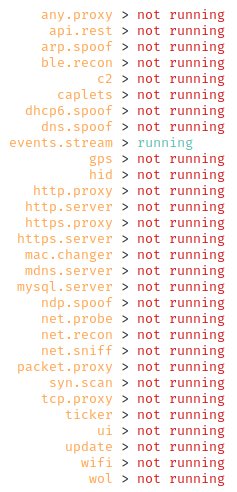
\includegraphics[width=4.5cm]{img/bettercap_help.png}
 % bettercap_help.png: 237x492 px, 96dpi, 6.27x13.02 cm, bb=0 0 178 369
 \caption{Bettercap help page}
 \label{fig: bettercap help}
\end{figure}

Every tool is called a caplet, we'll be using the ``https.proxy'' and ``arp.spoof'' caplets.

\pagebreak

\subsection{Setting up ARP Spoofing}

Once bettercap has been launched, to start ARP spoofing we just need to enter \verb|arp.spoof on| in the console.

By default the tool will send a spoofed ARP message with the attacker's IP address associated to the LAN Gateway every second to the entire subnet where the attacker is connected.

The configurable options are\cite{arp-poof-source-code}:

\begin{itemize}
 \item  \verb|arp.spoof.fullduplex| : If true, both the targets and the gateway will be attacked, otherwise only the target (if the router has ARP spoofing protections in place this will make the attack fail). (default=false)
 \item     \verb|arp.spoof.internal |: If true, local connections among computers of the network will be spoofed, otherwise only connections going to and coming from the external network. (default=false)
 \item \verb|arp.spoof.skip\_restore |: If set to true, targets arp cache won't be restored when spoofing is stopped. (default=false)
 \item      \verb|arp.spoof.targets |: Comma separated list of IP addresses, MAC addresses or aliases to spoof, also supports nmap style IP ranges. (default=<entire subnet>)
 \item    \verb|arp.spoof.whitelist |: Comma separated list of IP addresses, MAC addresses or aliases to skip while spoofing. (default=)
\end{itemize}

The results in the victim are the following:

\begin{figure}[!hb]
\centering
 \subfloat[ARP Table before Spoofing\label{fig: spoof-before}]{
 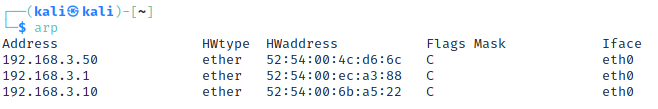
\includegraphics[width=7cm]{img/arp_spoof_before.png}}
 \vspace{0.5cm}
 \subfloat[ARP Table after Spoofing\label{fig: spoof-after}]{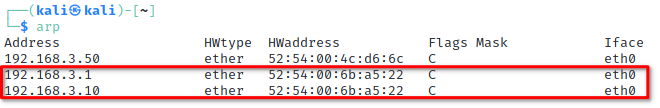
\includegraphics[width=7cm]{img/arp_spoof_after.png}}
 \caption{The result of ARP Spoofing/Poisoning}\label{fig: spoof-before-after}
\end{figure}

\pagebreak

Since the Gateway now points to the Attacker machine, the traceroute output is also changed:

\begin{figure}[!hb]
 \centering
 \subfloat[Traceroute before ARP Spoof\label{fig: traceroute-before}]{
 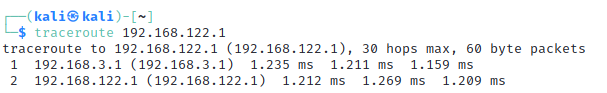
\includegraphics[width=7cm]{img/traceroute_before.png}}
 \vspace{0.5cm}
  \subfloat[Traceroute after ARP Spoof\label{fig: traceroute-after}]{
 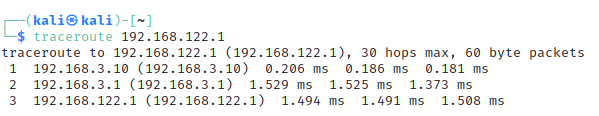
\includegraphics[width=7cm]{img/traceroute_after.png}}
\end{figure}


\subsection{Setting up the HTTPS Proxy}

As with the Arp Spoofer, launching the HTTPS Proxy through bettercap is similar.

The available options are:

\begin{itemize}
 \item \verb|https.port| : HTTPS port to redirect when the proxy is activated. (default=443)
 \item \verb|https.proxy.address| : Address to bind the HTTPS proxy to. (default=<interface address>)
 \item \verb|https.proxy.blacklist| : Comma separated list of hostnames to skip while proxying (wildcard expressions can be used). (default=)
 \item \verb|https.proxy.certificate| : HTTPS proxy certification authority TLS certificate file. (default=~/.bettercap-ca.cert.pem)
 \item \verb|https.proxy.certificate.bits| : Number of bits of the RSA private key of the generated HTTPS certificate. (default=4096)
 \item \verb|https.proxy.certificate.commonname| : Common Name field of the generated HTTPS certificate. (default=Go Daddy Secure Certificate Authority - G2)
 \item \verb|https.proxy.certificate.country| : Country field of the generated HTTPS certificate. (default=US)
 \item \verb|https.proxy.certificate.locality| : Locality field of the generated HTTPS certificate. (default=Scottsdale)
 \item \verb|https.proxy.certificate.organization| : Organization field of the generated HTTPS certificate. (default=GoDaddy.com, Inc.)
 \item \verb|https.proxy.certificate.organizationalunit| : Organizational Unit field of the generated HTTPS certificate. \newline(default=https://certs.godaddy.com/repository/)
 \item \verb|https.proxy.injectjs| : URL, path or javascript code to inject into every HTML page. (default=)
 \item \verb|https.proxy.key| : HTTPS proxy certification authority TLS key file. (default=~/.bettercap-ca.key.pem)
 \item \verb|https.proxy.port| : Port to bind the HTTPS proxy to. (default=8083)
 \item \verb|https.proxy.redirect| : Enable or disable port redirection with iptables. (default=true)
 \item \verb|https.proxy.script| : Path of a proxy JS script. (default=)
 \item \verb|https.proxy.sslstrip| : Enable or disable SSL stripping. (default=false)
 \item \verb|https.proxy.whitelist| : Comma separated list of hostnames to proxy if the blacklist is used (wildcard expressions can be used). (default=)
\end{itemize}

As mentioned earlier in the paper, the certificate can be forged meticulously to look like a big corporation's one.

\pagebreak

\subsubsection{Developing the Script}

Through the \verb|https.proxy.script| option, it is possible to develop a small javascript program that interacts with various proxy functions\cite{proxy-functions}:

\begin{verbatim}
 // called when the script is loaded
function onLoad() {

}

// called when the request is received by the proxy
// and before it is sent to the real server.
function onRequest(req, res) {

}

// called when the request is sent to the real server
// and a response is received
function onResponse(req, res) {

}

// called every time an unknown session command is typed,
// proxy modules can optionally handle custom commands this way:
function onCommand(cmd) {
    if( cmd == "test" ) {
        /*
         * Custom session command logic here.
         */

        // tell the session we handled this command
        return true
    }
}
\end{verbatim}

\pagebreak

In this case in order to bypass the Malware Detection in ``PanOS'', a small script was created that replaces the url of the malware on the external server with the url of the same malware but located on the attacker's machine.

\begin{verbatim}
function onResponse(req, res){
        var body = res.ReadBody();
        //Checks if there's a link to eicar.com
        if ( body.indexOf('<a href="./eicar.com">') != -1){
            res.Body = body.replace('<a href="./eicar.com">',
            '<a href="http://192.168.3.10/eicar2.com">');
        }
}
\end{verbatim}


\begin{figure}[h!]
 \centering
 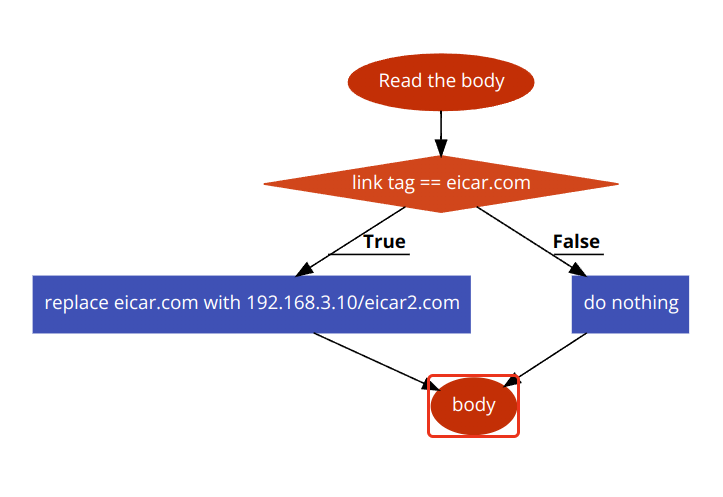
\includegraphics[width=13cm]{img/script_flowchart.png}
 % script_flowchart.png: 723x497 px, 96dpi, 19.13x13.15 cm, bb=0 0 542 373
 \caption{The Script's Flowchart}
 \label{fig: flowchart}
\end{figure}

\pagebreak

\subsubsection{Testing the Proxy}

Once the script has been written, to load it into the https.proxy the command \verb|set https.proxy.script /file/location/script.js`| is used in the bettercap shell and the proxy itself is started through the \verb|https.proxy on| command.

When loaded, once the client connects to the web server the SSL/TLS certificate will also have changed.

\begin{figure}[h!]
 \centering
 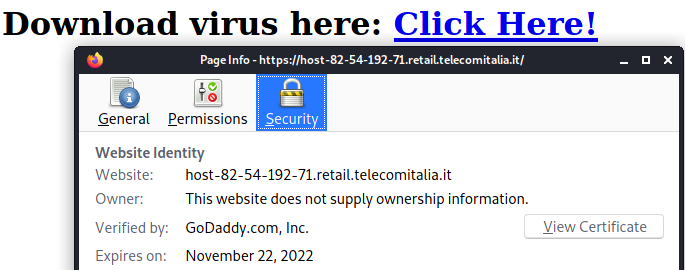
\includegraphics[width=13cm]{img/spoofed_certificate.png}
 % spoofed_certificate.png: 685x270 px, 96dpi, 18.12x7.14 cm, bb=
 \caption{The compromised website along with its forged Certificate}
 \label{fig: spoofed-certificate}
\end{figure}

And by Clicking the link the download will start as envisioned.

\begin{figure}[h!]
 \centering
 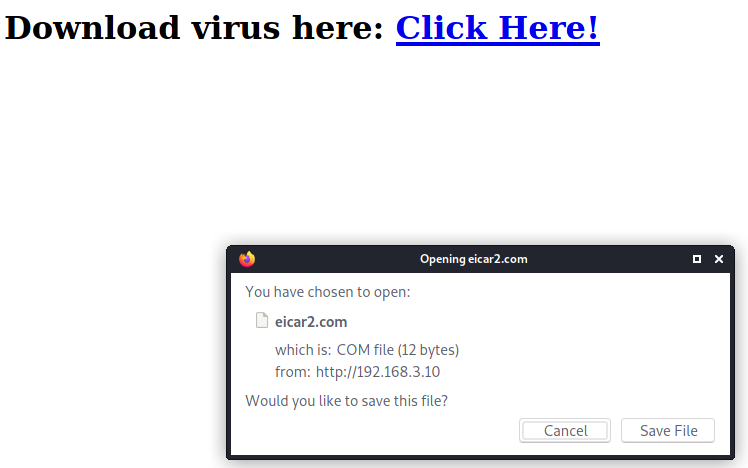
\includegraphics[width=13cm]{img/after_proxy.png}
 % after_proxy.png: 748x468 px, 96dpi, 19.79x12.38 cm, bb=
\end{figure}

This way the victim is downloading a malware by completely bypassing the Malware Detection system in the firewall.


\pagebreak

\section{Mitigating the Attack}


\chapter{Results and discussion}
\section{Conclusions}

\addcontentsline{toc}{chapter}{Bibliography}
\bibliography{bib/bib-latex,bib/bib-sample}
\bibliographystyle{ieeetr} % acm siam abbrv plain, alpha, abbrv, ieeetr

% --- list of tables and figures (indice delle tabelle, figure) ------------
\addcontentsline{toc}{chapter}{\listfigurename}
\ListOfFigures  % genera elenco e aggiunge voce all'indice(nella lingua corretta)


\PrintIndex % genera indice analitico, aggiunge voce all'indice (nella lingua corretta)
%\clearpage \addcontentsline{toc}{chapter}{Indice analitico} \printindex


\end{document}
